\section{Phase Characterization}

Phases can be characterized in many ways (e.g. phase duration, performance, power utilization, etc). For the SFG phases that we are studying, we look at the phase length, phase transitions, and phase coverage. The phase length is an important characteristic to consider because it guides the client's decision to apply an optimization that makes sense given the amount of time the phase will last for. Ideally, the phase will last long enough to amortize the cost for applying the new configuration. The phase transitions is important to consider since it may factor into the explore time overhead, which is the period when the client recognizes a phase shift and explores different configurations. Consecutive phase transitions that result in the same configuration by the client wastes the time and resources in exploring. A lower number of phase transitions is ideal along with only phase transitions that are significant enough to require a new configuration. The phase coverage is the percentage of the application that has been classified as in-phase as opposed to in transition. The higher the phase coverage, the more impact an optimization applied by the client can have on the code as a whole. While there are several other phase characteristics, we select to study phase length, phase transition, and phase coverage since they are critical characteristics that commonly factor into a cost-benefit analysis made by the client.       

\subsection{Phase Length}
Here, we analyze how the phase length changes as parameters such as the model, interval size, and similarity threshold varies. The \emph{low} threshold value ($t$) is set to $t=0.1$ and the \emph{high} threshold value is set to $t=0.9$. When otherwise not noted, $t=0.1$. The computed similarity values $s$ has range $0 \leq s \leq 1.0$, where $0$ indicates intervals that are perfectly similar and $1$ indicates intervals that are not at all similar. If a computed similarity value falls below the threshold, then the tested intervals are considered similar enough to form a phase. The interval size $i$ we allow to vary between 1 and 100K. The evaluated models include instruction working sets (IWS), basic block vectors (BBV), Intel Top Down (ITD), and CPI. 

\begin{figure}[htbp]
  \begin{center}
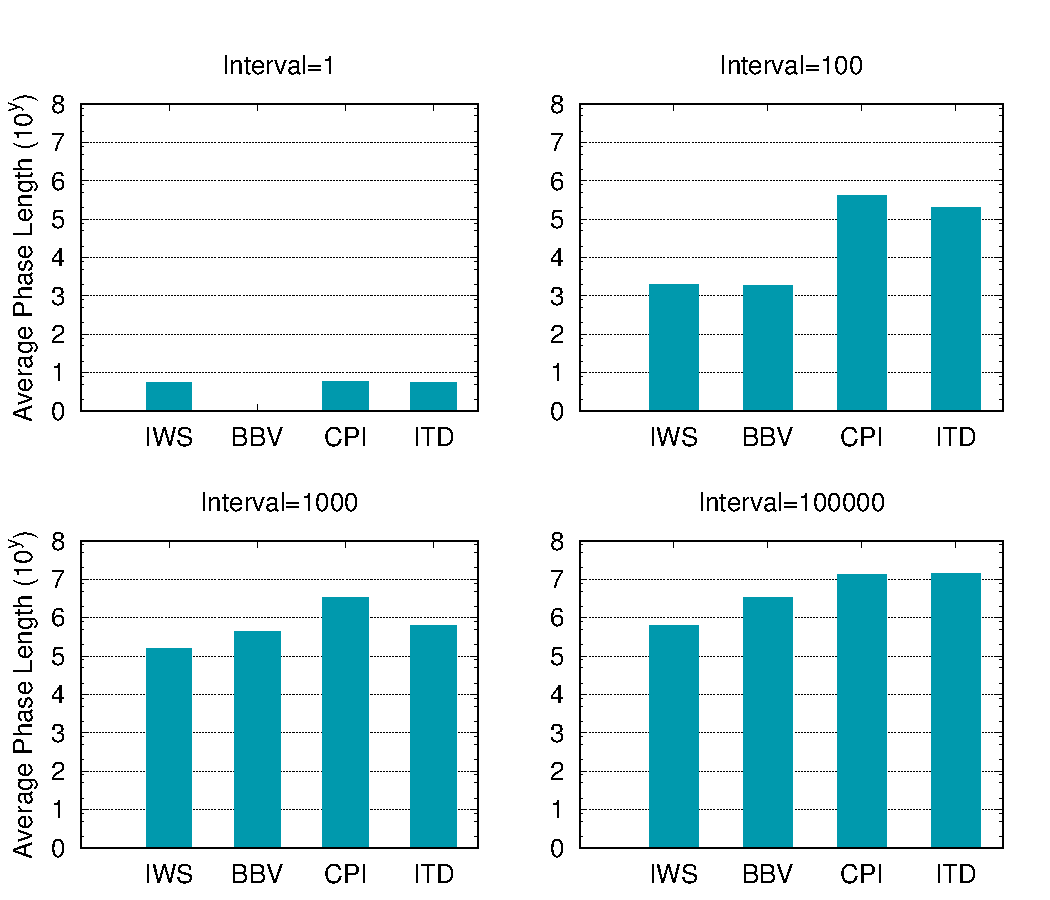
\includegraphics[width=0.99\columnwidth]{figs/phaselenavg}
  \end{center}
  \caption{At very short intervals, the phase lengths are similar across models. At longer intervals, differences in phase length begins to emerge between models.}
  \label{fig:phaselenavg}
\end{figure}

Figure~\ref{fig:phaselenavg} shows the absolute average phase length across different models and interval sizes. The range in phase length that can be observed is roughly 5-10M cycles long. The phases detected on the lower end of the size spectrum would be undetectable had the interval size been restricted to be much higher (e.g. 1M cycles). Another key observation is that the model deployed along with the interval size can have a significant effect on the phase length.  At an interval size of one cycle, we see little differences in the average phase length, which turns out to be roughly five cycles across models. As the interval size increases, we begin to see more separation with respect to the phase length across models. At an interval size of 100, both CPI and ITD have average phase lengths a couple of orders of magnitude higher then IWS and BBV. At even higher interval sizes, up to 100K, we still see some differences between models (about one order of magnitude difference). The interval size and model should be appropriately configured by the client to produce the desired phase length.

Figure~\ref{fig:phaselen} shows how the average phase length changes across the nine benchmarks as we vary all three parameters (interval size, model, and similarity threshold). One clear trend is that the phase length tends to grow as the interval size is increased. The growth rate is fast at smaller interval sizes and slows down at larger interval sizes. With respect to the similarity threshold, we see a much more pronouced growth in phase length at smaller interval sizes for higher threshold values. Along the same vein, we also generally see a much more pronounced slowdown of the growth in phase length at a higher threshold and interval size. Also note from Figure~\ref{fig:phaselen} the difference in phase length across the models. ITD tends to track more closely to CPI while IWS and BBV is tracking more closely with respect to phase length. Another interesting observation is that both CPI and ITD tend to have longer phase lengths with the former having the longest phase length, but this gap narrows given a higher threshold and interval size. To summarize, we observe the following trends with respect to phase length:

\begin{enumerate}
\item The phase length increases as the interval size increases.
\item The phase length increases at a faster rate given a higher threshold.
\item ITD tends to have a longer phase length compared to IWS and BBV and tracks more closely to CPI.
\end{enumerate}

The phase length as previously mentioned is of interest to the client in order to perform a cost benefit analysis of applying a new configuration. As Figure~\ref{fig:phaselen} shows, all three parameters (interval size, model, and similarity threshold) can impact the phase length and can be tweaked by the client in order to obtain the desired length. If a client desires a longer phase length, then that can be accomplished by increasing the interval size, relaxing the threshold, or switching models. The design of a phase analysis framework should enable the client to easily adjust these parameters to achieve the desired phase length. 


\begin{figure}[htbp]
  \begin{center}
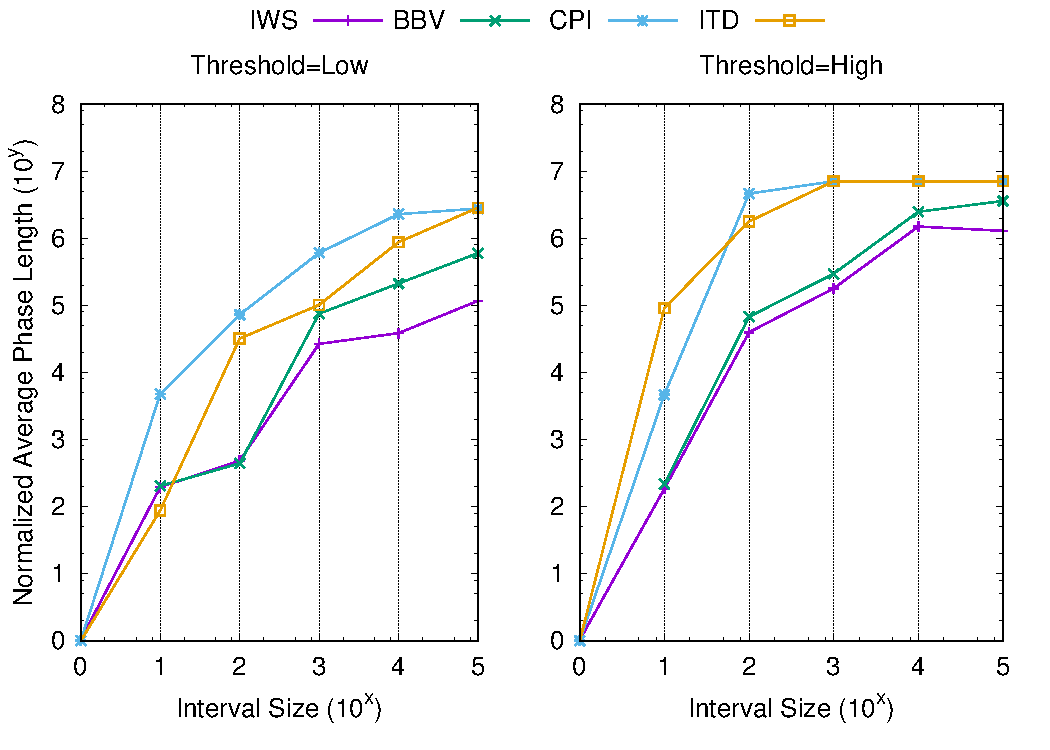
\includegraphics[width=0.99\columnwidth]{figs/phaselenfixthreshold}
  \end{center}
  \caption{All three parameters (interval size, model, and threshold) appear to have a significant effect on the phase length.}
  \label{fig:phaselen}
\end{figure}




\subsection{Phase Transitions}
Similar to the phase length analysis, we also vary the interval size, model, and similarity threshold and evaluate changes in phase transitions. As Figure~\ref{fig:phasetransavg} shows, as the interval size increases, the number of phase transitions tend to decrease. At higher thresholds, we see a separation in phase transition between IWS/BBV and ITD/CPI. Recall that in the phase length analysis, ITD tracked pretty closely with CPI as well and IWS and BBV tracked closely with each other. There appears to be a stabilization in the number of phase transitions at an interval size of 100 for the high threshold case for ITD and CPI, which coincides with the point at which the phase length for ITD and CPI begins to stabilize with increasing interval size as shown in Figure~\ref{fig:phaselen}. This suggests that increasing the interval size has the joint effect of increasing the phase length and decreasing the number of phase transitions, but that there does exist a stabilization point for which there will be little change in phase length and phase transitions. At low thresholds, we see very similar behavior in phase transition across models. In general, if a reconfiguration client is interested in lowering exploration costs by decreasing the number of phase transitions, it appears that the best avenue is to increase the interval size, but to also recognize there exists a limit as the number of phase transitions reaches it's minimum value and phase length reaches it's maximum value (i.e. a phase can not last longer then the duration of the program).  At higher thresholds, this stabilization in phase transitions and phase length occurs at a much earlier point as the interval size increases. 

\begin{figure}[htbp]
  \begin{center}
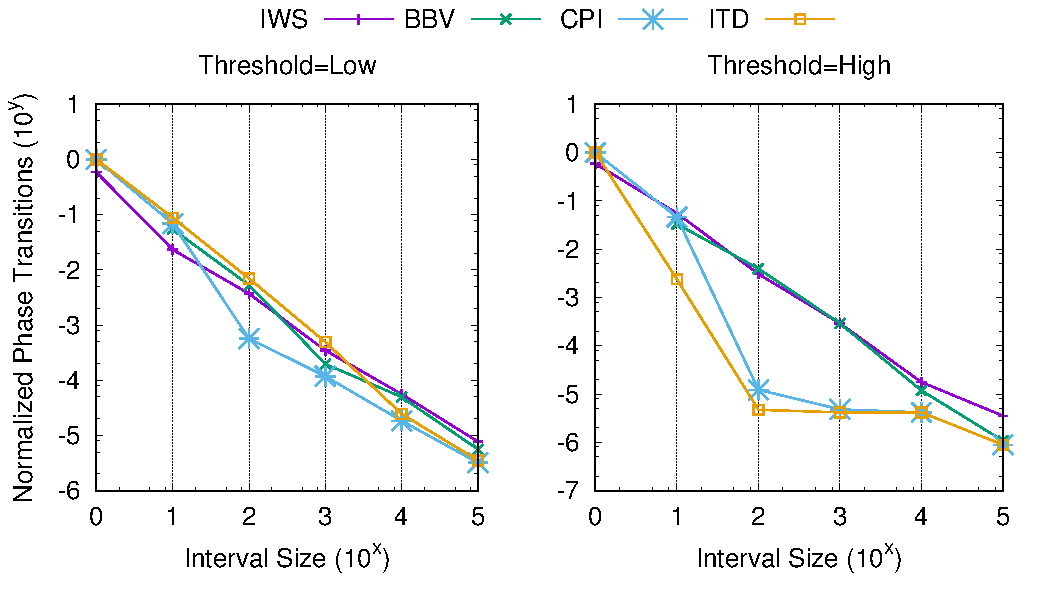
\includegraphics[width=0.95\columnwidth]{figs/phasetransavg}
  \end{center}
  \caption{The interval size is the most effective parameter for varying the phase transition compared with the model and threshold. But the threshold value does impact the rate at which the phase transitions decrease as the interval size grows and this behavior appears to vary between models.}
  \label{fig:phasetransavg}
\end{figure}





\subsection{Phase Coverage}
The phase coverage determines the proportion of the program where phase behavior has been defined. Periods of execution where phase behavior has not been defined is considered to be phase transition periods. The phase coverage determines the percentage of the application that can benefit from some client-side optimization and so ideally a high level of phase coverage is preferable. 

Figure~\ref{fig:phasecycles} shows that the phase coverage is not very well behaved with respect to the interval size. That is, as the interval size increases, there is no clear trend in phase coverage. By contrast, there does appear to be some consistent trends for phase coverage with respect to the threshold and model. A higher threshold appears to increase the phase coverage. CPI followed closely by ITD also appears to have higher phase coverage compared to IWS and BBV, with IWS generally having the lowest phase coverage. As far as configuration clients are concerned, adjusting the model as well as increasing the similarity threshold should effectively increase the phase coverage.

\begin{figure}[htbp]
  \begin{center}
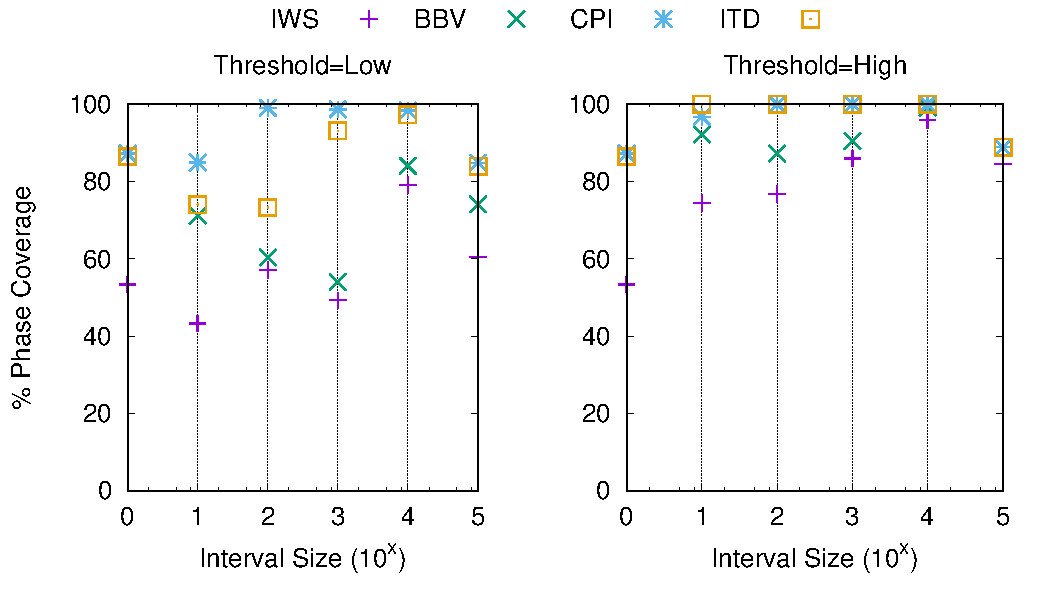
\includegraphics[width=0.99\columnwidth]{figs/phasecyclesthreshold}
  \end{center}
  \caption{Increasing the similarity threshold and using particular models (such as ITD) will tend to result in higher phase coverage.}
  \label{fig:phasecycles}
\end{figure}


